\secframe{SquirrelMail}{
    Web-Adressen f\"ur den Webmailer\footnote{\url{https://squirrelmail.org}}\footnote{\url{https://squirrelmail.org/docs/user/user.html}}.
	\begin{description}
		\item[allg.] \url{https://webmail.htw-dresden.de}
		\item[Info/Mathe] \url{https://webmail.informatik.htw-dresden.de}
		\item[WiWi] \url{https://webmail.wiwi.htw-dresden.de}
	\end{description}
   \begin{figure}
	   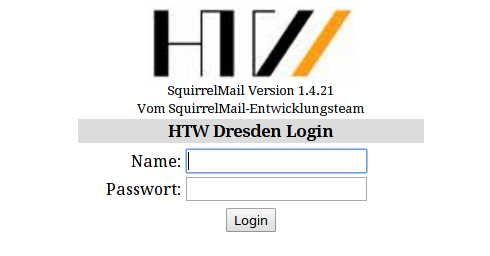
\includegraphics[width=0.7\textwidth]{../images/wm_loginseite.png}
   \end{figure}
}

\frame{
	\frametitle{SquirrelMail Startseite}
   \begin{figure}
	   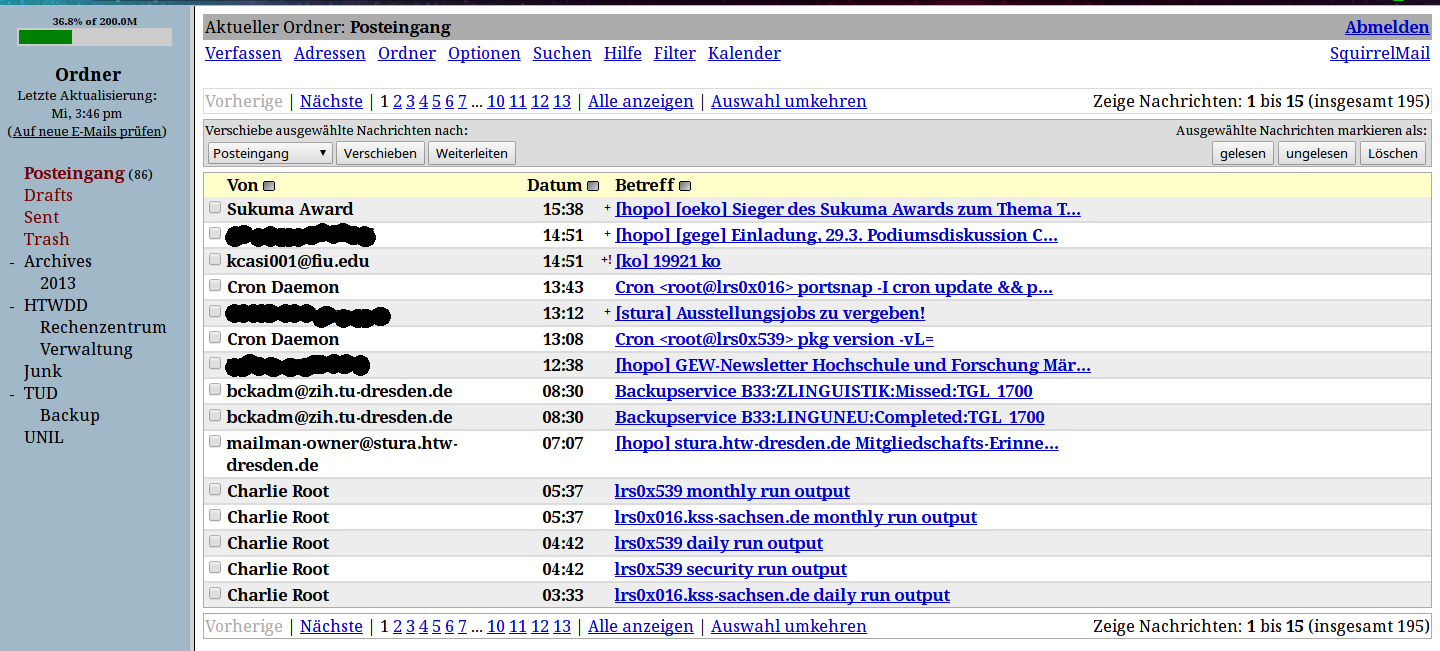
\includegraphics[width=\textwidth]{../images/wm_startseite.png}
   \end{figure}
}

\frame{
	\frametitle{SquirrelMail Startseite II}
	Nach dem Login erh\"alt man eine \"Ubersicht der empfangen Mails und kann im oberen Bereich folgende Funktionen w\"ahlen:
	\begin{description}
		\item[Verfassen] E-Mail schreiben
		\item[Adressen] Zum Adressbuch hinzuf\"ugen, importieren/exportieren
		\item[Ordner] erstellen/umbenennen/l\"oschen/austragen der eintragen
		\item[Optionen] Manage Identities/Farbthema
		\item[Suchen] Ornder durchsuchen
		\item[Hilfe] FAQ
		\item[Filter] Filterregeln (de)aktivieren/erstellen
		\item[Kalender] Kalender/Termine
	\end{description}
	}

\subsecframe{Ordner}{
        \begin{columns}
            \begin{column}{0.75\textwidth}
                \begin{figure}
	   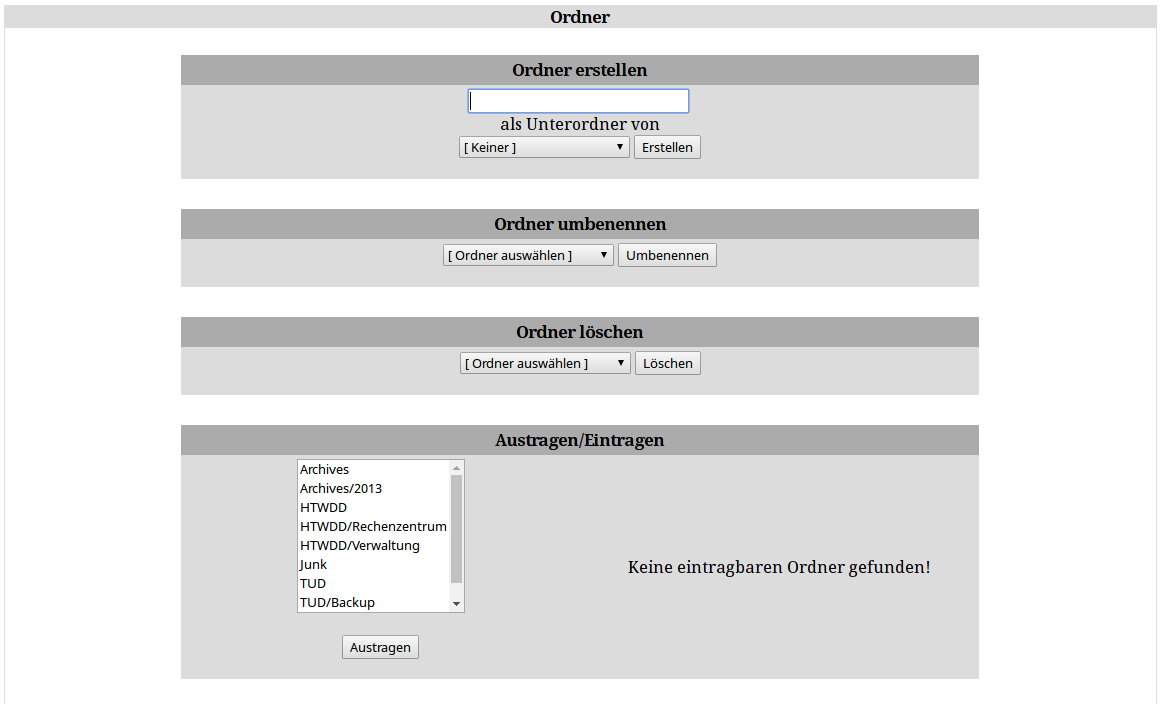
\includegraphics[width=\textwidth]{../images/wm_ordner.png}
                \end{figure}
            \end{column}
            \begin{column}{0.4\textwidth}  %%<--- here
	\begin{itemize}
		\item erstellen
		\item umbenennen
		\item l\"oschen
		\item austragen/eintragen
	\end{itemize}
            \end{column}
        \end{columns}
	}

\subsecframe{Manage Identities / Aliases}{
    \centering
    \begin{columns}
        \begin{column}{0.50\textwidth}
            \begin{figure}
                1.
                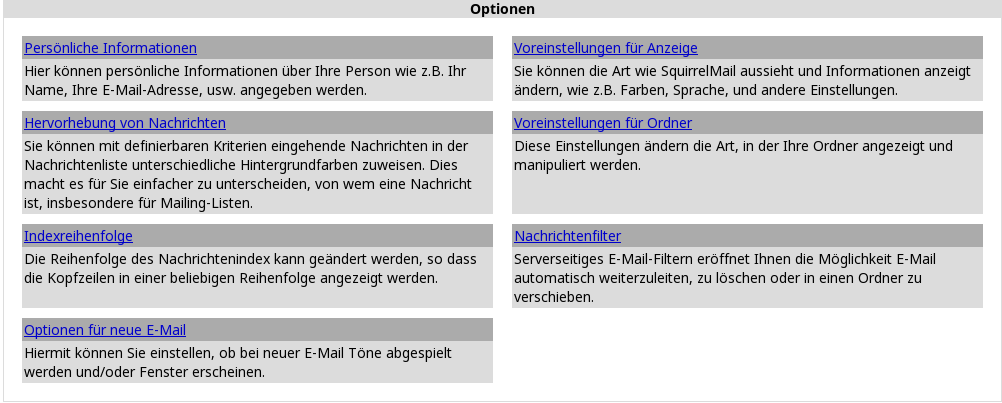
\includegraphics[width=\textwidth]{../images/wm_options.png}
            \end{figure}
            \begin{figure}
                2.
                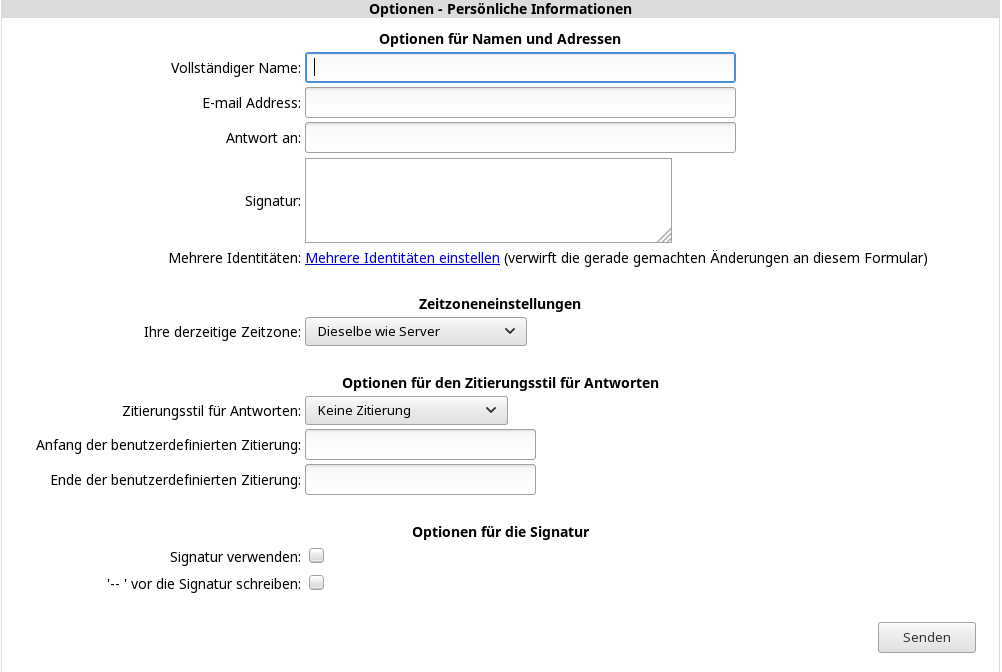
\includegraphics[width=\textwidth]{../images/wm_priv_info.png}
            \end{figure}
        \end{column}
        \begin{column}{0.50\textwidth}
            \begin{figure}
                3.
                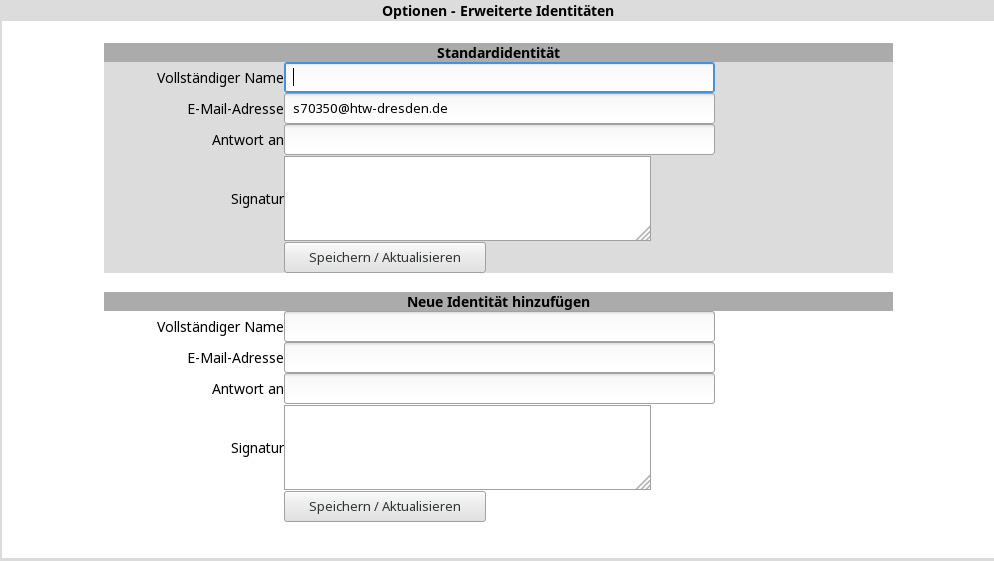
\includegraphics[width=\textwidth]{../images/wm_aliases.png}
            \end{figure}
            \begin{description}
                \item[1.] Optionen
                \item[2.] Pers\"onliche Informationen
                \item[3.] Mehrere Identit\"aten einstellen
            \end{description}
        \end{column}
    \end{columns}
}

\subsecframe{Manage Identities / Aliases II}{
                \begin{figure}
                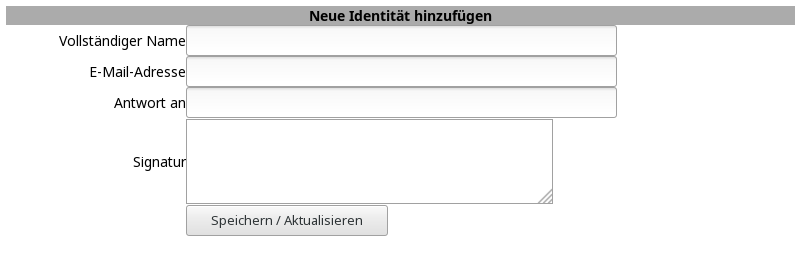
\includegraphics[width=\textwidth]{../images/wm_new_alias.png}
                \end{figure}
        \begin{columns}
            \begin{column}{\textwidth}
                \begin{description}
                    \item[Vollst\"andiger Name:] $<$Vorname$>$ $<$Nachname$>$ / $<$Funktion$>$
                    \item[E-Mail-Adresse:] $<$Nachname/Funktion$>$@stura.htw-dresden.de
                    \item[Antwort an:] $<$E-Mail-Adresse$>$
                    \item[Signatur:] $<$Vorname$>$ $<$Nachname$>$ / $<$Funktion$>$\newline
                    \newline
                    StuRa HTW Dresden\newline
                    Andreas-Schubert-Str. 23\newline
                    01069 Dresden
                \end{description}
            \end{column}
        \end{columns}
}
\subsecframe{Filter} {
	\begin{itemize}
		\item aktivieren
		\item deaktivieren
		\item hinzuf\"ugen
		\item bearbeiten/kopieren/l\"oschen
	\end{itemize}
   \begin{figure}
	   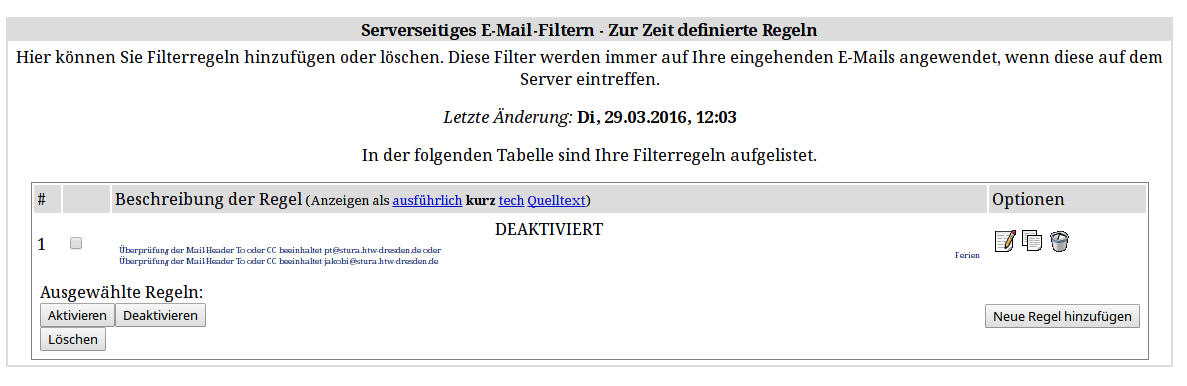
\includegraphics[width=\textwidth]{../images/wm_filterseite.png}
   \end{figure}
}

\frame{
	\frametitle{Filter II}
   \begin{figure}
	   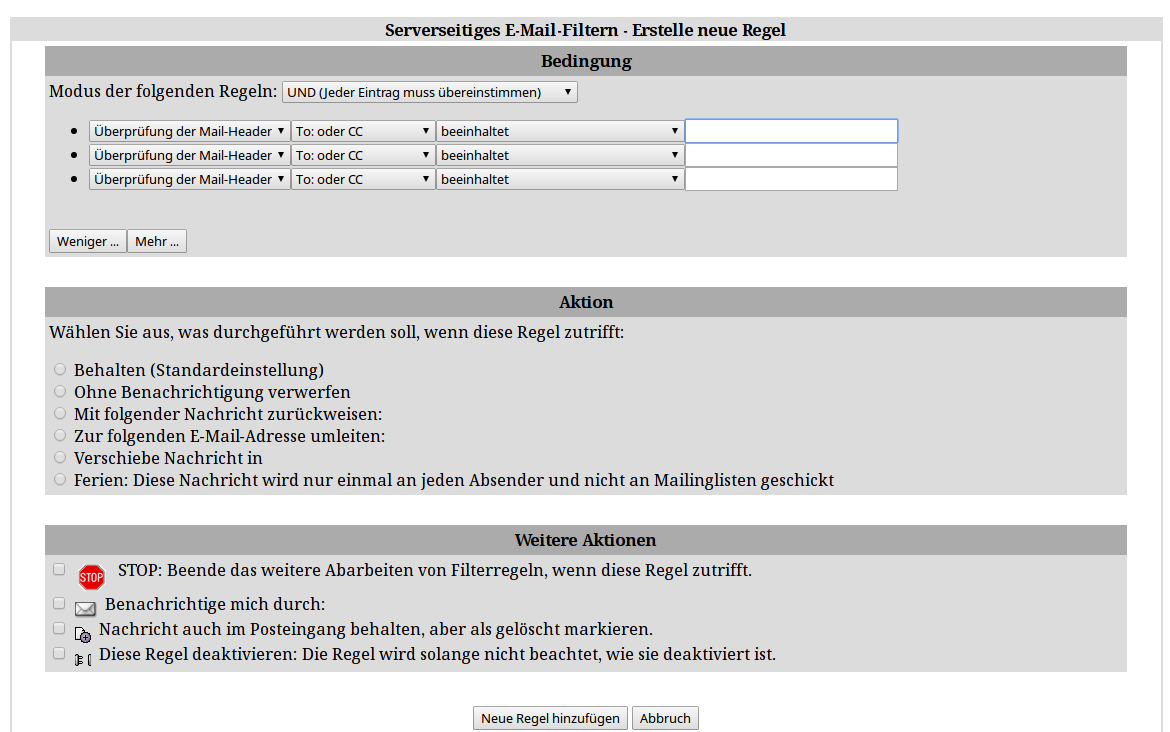
\includegraphics[width=\textwidth]{../images/wm_neue_filter_regeln.png}
   \end{figure}
   }

   \frame{
       \frametitle{Spamfilter I}
       \begin{figure}
           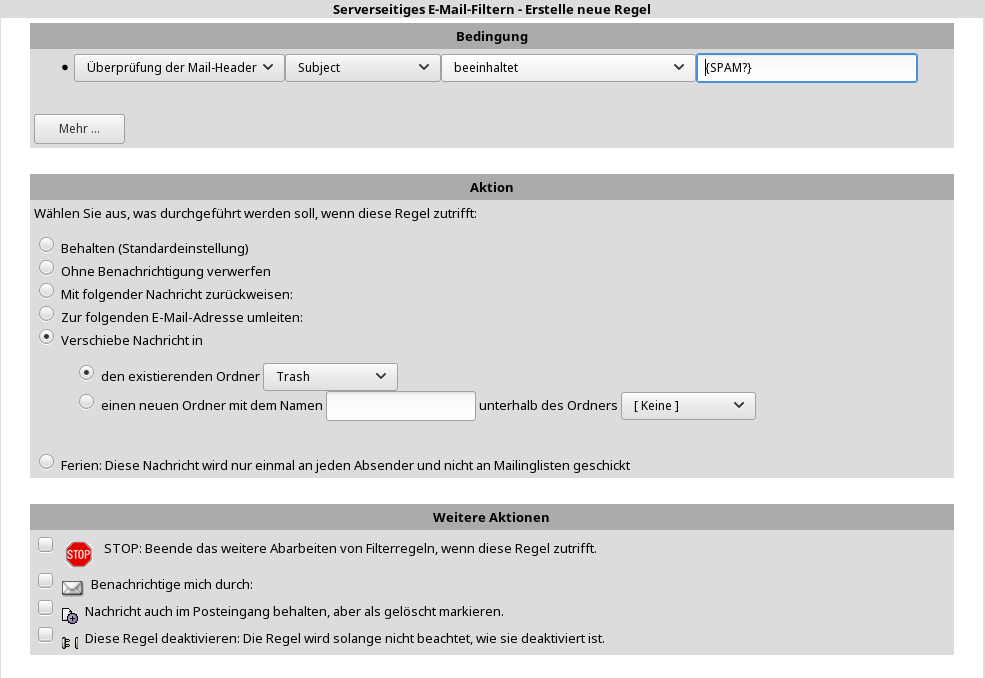
\includegraphics[width=\textwidth]{../images/wm_spamilter.png}
       \end{figure}
   }
   \frame{
       \frametitle{Spamfilter II}
       \begin{itemize}
           \item \textbf{Bedingung}
               \begin{itemize}
                   \item \textit{\"Uberpr\"ufung der Mail-Header}
                   \item \textit{Subject}
                   \item \textit{beeinhaltet}\footnote{Typo Fehler wurde \"ubernommen!}
                   \item \textit{$\{SPAM?\}$}
               \end{itemize}
           \item \textbf{Aktion}
               \begin{itemize}
                   \item Verschiebe Nachricht in
                       \begin{itemize}
                           \item den existierenden Ordner \textit{Trash}
                       \end{itemize}
               \end{itemize}
       \end{itemize}
   }
